% Exemplo de relatório técnico do IC

% Criado por P.J.de Rezende antes do Alvorecer da História.
% Modificado em 97-06-15 e 01-02-26 por J.Stolfi.
% modificado em 2003-06-07 21:12:18 por stolfi
% modificado em 2008-10-01 por cll
% modificado em 2010-03-16 17:56:58 por stolfi
% modificado em 2012-09-25 para ajustar o pacote UTF8. Contribuicao de Rogerio Cardoso
% \def\lastedit{2015-03-18 00:52:20 by bit}

\nonstopmode % PARA RODAR LATEX EM BATCH MODE
\documentclass[11pt,twoside]{article}

\usepackage{techrep-ic}
\usepackage{amsmath}
\usepackage{amssymb}
\usepackage{subcaption}
\usepackage[english]{babel}
\usepackage[utf8]{inputenc}
\usepackage[margin=1in]{geometry}
\usepackage[
  style=numeric,
  sorting=none
]{biblatex}
\addbibresource{references.bib}
\usepackage{xcolor}
\usepackage[hidelinks]{hyperref}
\usepackage[noabbrev, capitalise]{cleveref}
\usepackage[cache=false]{minted}
\usemintedstyle{borland}

\begin{document}

%%% PÁGINA DE CAPA %%%%%%%%%%%%%%%%%%%%%%%%%%%%%%%%%%%%%%%%%%%%%%%
% 
% Número do relatório
\TRNumber{41} % Dois dígitos
\TRYear{23} % Dois dígitos
\TRMonth{12} % Numérico, 01-12
\TRAuthor{Paulo Pacitti \and Julio López}
\TRTitle{Software implementation of Ascon on the 64-bit RISC-V Allwinner D1 processor}
\TRMakeCover

%%%%%%%%%%%%%%%%%%%%%%%%%%%%%%%%%%%%%%%%%%%%%%%%%%%%%%%%%%%%%%%%%%%%%%
% O que segue é apenas uma sugestão - sinta-se à vontade para
% usar seu formato predileto, desde que as margens tenham pelo
% menos 25mm nos quatro lados, e o tamanho do fonte seja pelo menos
% 11pt. Certifique-se também de que o título e lista de autores
% estão reproduzidos na íntegra na página 1, a primeira depois da
% página de capa.
%%%%%%%%%%%%%%%%%%%%%%%%%%%%%%%%%%%%%%%%%%%%%%%%%%%%%%%%%%%%%%%%%%%%%%

%%%%%%%%%%%%%%%%%%%%%%%%%%%%%%%%%%%%%%%%%%%%%%%%%%%%%%%%%%%%%%%%%%%%%%
% Nomes de autores ABREVIADOS e titulo ABREVIADO,
% para cabeçalhos em cada página.
%
\markboth{Pacitti, López}{Software implementation of Ascon on the 64-bit RISC-V Allwinner D1 processor}
\pagestyle{myheadings}
\thispagestyle{empty}

%%%%%%%%%%%%%%%%%%%%%%%%%%%%%%%%%%%%%%%%%%%%%%%%%%%%%%%%%%%%%%%%%%%%%%
% TÍTULO e NOMES DOS AUTORES, completos, para a página 1.
% Use "\\" para quebrar linhas, "\and" para separar autores.
%
\title{Software implementation of Ascon on \\ the 64-bit RISC-V Allwinner D1 processor}

\author{Paulo Pacitti\thanks{Institute of Computing, UNICAMP. \texttt{p185447@dac.unicamp.br}} \and
  Julio  López\thanks{Associate Professor, Institute of Computing, UNICAMP. \texttt{jlopez@ic.unicamp.br}}}
\date{}
\maketitle

%%%%%%%%%%%%%%%%%%%%%%%%%%%%%%%%%%%%%%%%%%%%%%%%%%%%%%%%%%%%%%%%%%%%%%

\begin{abstract}
  RISC-V is a promising ISA and soon will be the architecture of many chips, specially embedded systems. It's necessary to guarantee that applications that run in systems designed with RISC-V will be at the same time secure and cryptographically fast. The NIST Lightweight Cryptography competition selected the finalist: Ascon, a family of cryptography algorithms designed to run in devices with low computational power. This research explores the Ascon family of algorithms in the RISC-V 64-bit architecture, analysing the Ascon permutation and the Ascon-128 algorithm, and whether it's possible to optimize it for \texttt{riscv64}, proposing a new technique regarding the decryption implementation. The results show that the proposed optimizations, developed during the limited time given to this research, were not enough to overcome all the implementations that were benchmarked. Finally, it's discussed that new microarchitectures, and, the future of the RISC-V ISA with new instructions extensions recently ratified, could improve the performance of the Ascon family of algorithms and other cryptographic algorithms.
\end{abstract}

\section{Introduction}
Inspired by the works of the UNICAMP's Laboratory of Security and Cryptography in the optimization of cryptographic algorithms for the ARM architecture \cite{Fujii2017a}, the NIST Lightweight Cryptography competition finalist algorithm \cite{turan2023status}, and the RISC-V open architecture, this research aims to explore the Ascon family of algorithms \cite{asconv12nist} on the RISC-V 64-bit architecture and whether it's possible to optimize it for this architecture. There are other works that have explored the Ascon family of algorithms on RISC-V, but in the 32-bit architecture and benchmarking in an FPGA chip. This research was done in the 64-bit RISC-V architecture and benchmarking it in a real chip, the Allwinner D1.

The approach was to analyse the Ascon algorithm design for three different implementations. All the implementations tested are written in C. The first implementation \texttt{ref} is the reference implementation of Ascon, written by Ascon team \cite{asconc2023}. The second one is \texttt{opt64}, an optimized implementation for a generic 64-bit architecture system, also developed by the Ascon team. The  third implementation was the main objective of this research, named \texttt{ascon-v} \cite{asconv2023}, this implementation is focused on producing an optimized version for the RISC-V 64-bit architecture, more specific, using only the instruction set \textsf{RV64GC}. The research was focused on trying to improve the basic blocks of the Ascon family of algorithms. Because of that, the analysis, optimizations, and results are focused on the \textsc{Ascon-128}, which is the \textit{de facto} authenticated encryption with associated data (AEAD) standard of the Ascon family.

\section{Ascon}

Ascon is a family of algorithms for lightweight cryptography, designed to be used in constrained environments, like embedding computing. Designed by cryptographers from Graz University of Technology, Infineon Technologies, Intel Labs, and Radboud University, Ascon has been selected as the new standard for lightweight cryptography in the 2019–2023 NIST Lightweight Cryptography competition. The Ascon family is mainly composed by 4 algorithms: \textsc{Ascon-128}, \textsc{Ascon-128a}, \textsc{Ascon-Hash} and \textsc{Ascon-Hasha}. There's also variants \textsc{Ascon-80pq}, \textsc{Ascon-Xof}, \textsc{Ascon-Xofa}, where the first it's a version of AEAD with an increased key size of 160 bits and the latter two are versions of the hash algorithm, but they produce hash outputs of arbitrary length.

The \cref{table:aeadParameters} shows the parameters of the recommended AEAD schemes from the Ascon family of algorithms, where this work will focus on the \textsc{Ascon-128}. The algorithms use the encryption function $\textit{E}_{k,r,a,b}$ and the decryption function $\textit{D}_{k,r,a,b}$ where $k$ is the key size, $r$ is the rate (data block) size, $a$ and $b$ are the number of rounds used in $p^a$ and $p^b$ permutations used across the algorithms. The encryption $\textit{E}_{k,r,a,b}(K, A, N, P) = (C, T)$ receives a key $K$, an associated data $A$, a nonce $N$ and a plaintext $P$ and returns a ciphertext $C$ and a tag $T$. The decryption $\textit{D}_{k,r,a,b}(K, A, N, C, T) \in \{P, \perp\}$ receives a key $K$, an associated data $A$, a nonce $N$, a ciphertext $C$ and a tag $T$ and returns the plaintext $P$ if the verification of the tag is correct, otherwise it returns the $\perp$ error.

\begin{table} [h]
  \centering
  \begin{tabular}{|c|c|cccc|cc|}
    \hline
    \textbf{Name}       & \textbf{Algorithms}                     & \textbf{key} & \textbf{nonce} & \textbf{tag} & \textbf{data block} & \textbf{$p^a$} & \textbf{$p^b$} \\ \hline
    \textsc{Ascon-128}  & \textit{E}, $\textit{D}_{128,64,12,6}$  & 128          & 128            & 128          & 64                  & 12             & 6              \\ \hline
    \textsc{Ascon-128}a & \textit{E}, $\textit{D}_{128,128,12,8}$ & 128          & 128            & 128          & 128                 & 12             & 8              \\ \hline
  \end{tabular}
  \caption{Ascon AEAD scheme parameters}
  \label{table:aeadParameters}
\end{table}

Ascon lightweight properties comes from using the simple bitwise operations that majority of microcontrollers have, like XOR, AND, OR, NOT, and bitwise rotations. The algorithm is based in the sponge construction, which is a cryptographic primitive that can be used to build cryptographic hash, encryption, and pseudorandom functions. The most known example of a cryptographic scheme that uses the sponge function is SHA-3 (also known as “Keccak”) \cite{bertoni2015keccak} algorithm. The sponge construction consists in keeping a finite internal state that takes input streams (absorb) to update the state and output streams (squeeze) to produce the output from the internal state. The Ascon state is composed by five 64-bit words, also named as Ascon words, resulting in a 320-bit internal state. This internal state is then manipulated using the Ascon permutation procedure.

\subsection{Permutation}

The Ascon permutation is the main building block of the Ascon family of algorithms and consists in 3 stages: round constant addition, a substitution-layer (S-Box) and a linear diffusion layer. It's then used in the AEAD encryption and decryption procedures in the form of $p^a$ and $p^b$, where $p$ is the permutation and $a$ and $b$ are the number of rounds used in different stages of the algorithm. The parameters $a$ and $b$ are different for each algorithm of the Ascon family, but the permutation is the same for all of them, as it's displayed in \cref{table:aeadParameters}.

As the Ascon state has five 64-bit words, the round constant addition consists in XORing the round constant with the third Ascon word. The round constant is a 64-bit value that is different for each round. The substitution-layer consists in applying an S-Box to the Ascon state. The 5-bit S-Box updates the state with 64 parallel applications of substitutions to the five Ascon words, as seen in \cref{fig:asconsbox}. The linear diffusion layer consists in the linear diffusion function $x_i \leftarrow \Sigma_i(x_i)$ applied to each Ascon word $x_i$, where each word has a specific function definition $\Sigma_i(x_i)$. The linear diffusion function definitions are shown in \cref{fig:asconlineardiffusion}.

\begin{figure}
  \centering
  \begin{subfigure}[b]{0.4\textwidth}
    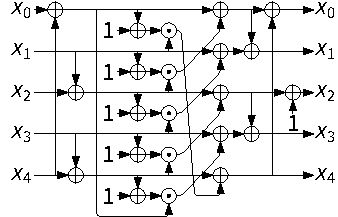
\includegraphics[scale=1]{assets/sbox.pdf} \\
    \caption{Ascon permutation S-box.}
    \label{fig:asconsbox}
  \end{subfigure}
  \hspace*{0.01\textwidth}
  \begin{subfigure}[B]{0.55\textwidth}
    \begin{align*}
       & x_0 \leftarrow \Sigma_{0}(x_0) = x_0 \oplus (x_0 \ggg 19) \oplus (x_0 \ggg 28)          \\
       & x_1 \leftarrow \Sigma_{1}(x_1) = x_0 \oplus (x_1 \ggg 61) \oplus (x_0 \ggg 39)          \\
       & x_2 \leftarrow \Sigma_{2}(x_2) = x_2 \oplus (x_2 \ggg \ \, 1) \oplus (x_2 \ggg \ \,  6) \\
       & x_3 \leftarrow \Sigma_{3}(x_3) = x_3 \oplus (x_3 \ggg 10) \oplus (x_3 \ggg 17)          \\
       & x_4 \leftarrow \Sigma_{4}(x_4) = x_4 \oplus (x_4 \ggg \ \,  7) \oplus (x_4 \ggg 41)
    \end{align*}
    \vspace*{0.07\textwidth}
    \caption{Ascon linear diffusion layer}
    \label{fig:asconlineardiffusion}
  \end{subfigure}
  \caption{S-box and linear diffusion layers in the Ascon permutation.}
  \label{fig:asconPermutation}
\end{figure}



\subsection{Encryption}

\begin{figure}[h]
  \centering
  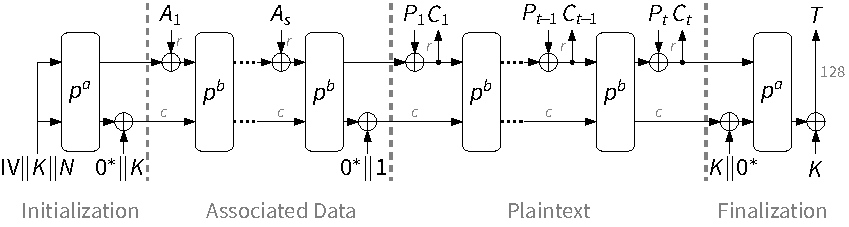
\includegraphics[scale=0.8]{assets/aead_encrypt.pdf}
  \caption{\textsc{Ascon-128} encryption scheme.}
  \label{fig:ascon128Encrypt}
\end{figure}


The AEAD encryption procedure in Ascon consists of three parts: initialization, associated data, plaintext processing and finalization. It's represented in \cref{fig:ascon128Encrypt}. In the initialization part, the Ascon state is defined by the bit string composed of the initialization vector, a key, and a nonce. The initialization vector is a combination of the parameters of the selected AEAD scheme. In the case of \textsc{Ascon-128}, $IV \leftarrow \texttt{0x80400c0600000000} $. After that, the Ascon $p^a$  permutation is applied and the Ascon state is XORed with the key $K$ padded with zeros in the beginning.

The associated data part consists in absorbing the associated data into the Ascon state. The associated data is absorbed in $r$-bit data blocks, where each block is XORed with the Ascon state and then the $p^b$ permutation is applied. The last block of the associated data is padded with the value 1 followed by zeros at the end, until it reaches the $r$-bits. At the end of the associated data processing part, the Ascon state absorbs a 320-bitstring of the value 1.

The plaintext processing part is where the ciphertext is generated. The plaintext is absorbed in the data blocks of size $r$, specified by the scheme parameters, where each block is XORed with the Ascon state, the state squeezes a ciphertext of same size, and, then, the Ascon $p^b$ permutation is applied. The last block of the plaintext $\tilde{P_t}$ is also XORed with the Ascon
state, but the squeezed ciphertext is $\tilde{C_t} \leftarrow {\left \lfloor  S_r \right \rfloor}_{|P| \ \textrm{mod} \ r}$.

The finalization part comprises the state being XORed with the key padded in the beginning with $r$ zeros and at the end with the remaining zeros to complete a 320-bit bit string, then applying the Ascon $p^a$ permutation to the Ascon state. To finish, the tag $T$ is generated by $T \leftarrow {\left \lceil  S \right \rceil}^{128} \oplus  {\left \lceil  S \right \rceil}^{128}$, and the algorithm returns the ciphertext $C$ and the tag $T$.

\subsection{Decryption}

\begin{figure}[h]
  \centering
  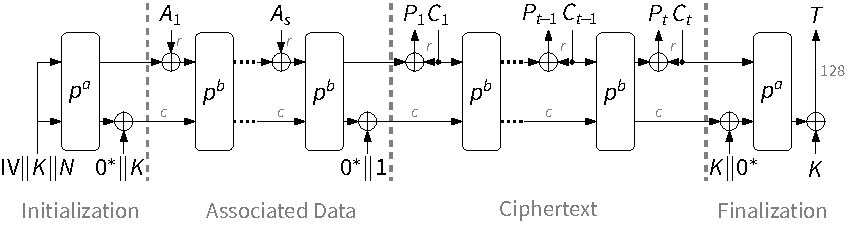
\includegraphics[scale=0.8]{assets/aead_decrypt.pdf}
  \caption{\textsc{Ascon-128} decryption scheme.}
  \label{fig:ascon128decrypt}
\end{figure}

The \textsc{Ascon-128} decryption has almost the same structure as seen in the encryption. The initialization and the associated data stages are the same as in the encryption. The ciphertext processing stage consists in absorbing (XORing with the first Ascon word) a ciphertext block $C_i$, squeeze  a block of the decrypted plaintext $P_i$, replace the first Ascon word $x_0$ with the current ciphertext block $C_i$, and then, permutate the Ascon state with $p^b$. The last block of the ciphertext $\tilde{C_t}$ is also absorbed in the Ascon state, but the squeezed plaintext is $\tilde{P_t} \leftarrow {\left \lfloor  S_r \right \rfloor}_{|C| \ \textrm{mod} \ r}$. After this, the first $r$ bits of the Ascon state is XORred with the bit string of the last deciphered plaintext concatenated with the value 1 and padded with zeros until it reaches the $r$ bits. In mathematical terms, these both operations can be seen in \cref{eq:2} and \cref{eq:3}.

The finalization stage is expressed by XORing the Ascon state with the key padded with $r$ zeros in the beginning and the remaining zeros at the end to complete a 320-bit bit string, then applying the Ascon $p^a$ permutation to the Ascon state. At the end, the tag $T$ is generated by $T \leftarrow {\left \lceil  S \right \rceil}^{128} \oplus  {\left \lceil  K \right \rceil}^{128}$, and the algorithm returns the plaintext $P$ if the verification of the tag is correct, otherwise it returns the $\perp$ error.

\section{Implementation and Optimizations}

The device used for this research is the MangoPi MQ-Pro, an SBC powered with an Allwinner D1 chip, 1 GB of DDR3 RAM, Wi-Fi, Bluetooth and HDMI video output. The Allwinner D1 chip contains a T-Head Xuantie C906 core, a RISC-V 64-bit 1 GHz single-issue CPU supporting \textsf{RV64GC} ISA. The instruction set \textsf{RV64GC} is equivalent to the \textsf{RV64IMAFDCZicsr\_Zifencei} set of extensions, where \textsf{I} stand for the Integer instruction set, \textsf{M} for multiplication, \textsf{A} for atomic, \textsf{F} for Single-Precision Floating-Point, \textsf{D} for Double-Precision Floating-Point, \textsf{C} for compressed, \textsf{Zicsr} for Control and Status Register (CSR), and \textsf{Zifencei} for Instruction-Fetch Fence. The board runs Ubuntu Server 23.04, running the 6.2.0-36-generic version of the Linux kernel. For compiling the implementation in C, it was used the RISC-V GNU Compiler Collection (GCC) version 12.2.0 \cite{riscvgnutoolchainv2023} through cross-compilation with Newlib, using a MacBook Pro with an Apple M1 chip. The implementation techniques that are going to be described next were used in the \texttt{asconv} implementation to attempt to overcome the performance of \texttt{ref} and \texttt{opt64} implementations.

Since it's a 64-bit architecture, it's possible to store each of the five 64-bit Ascon words in one register at a time. The use of the library \texttt{<stdint>} becomes very useful since it's possible to define exactly the bit string size representation, not being dependent on what the C types \texttt{long long} and \texttt{unsigned long long} translates to in a given machine. The Ascon permutation S-box seen in \cref{fig:asconsbox} translates to what it can be seen in the \cref{lst:1}, as well the round constant addition and linear diffusion stages (\cref{fig:asconlineardiffusion}).

\begin{listing}[ht!]
  \begin{minted}{c}
    // Ascon state with 5 64-bit words.
    typedef struct {
        uint64_t x[5];
    } ascon_state_t;

    // Bitwise rotation to the right.
    static inline uint64_t ROR(uint64_t x, int n) {
        return x >> n | x << (-n & 63);
    }

    // Ascon permutation round function.
    static inline void ROUND(ascon_state_t *s, const uint8_t C) {
        ascon_state_t t;
        /* round constant layer */
        s->x[2] ^= C;
        /* substitution layer */
        s->x[0] ^= s->x[4];
        s->x[4] ^= s->x[3];
        s->x[2] ^= s->x[1];
        t.x[0] = s->x[0] ^ (~s->x[1] & s->x[2]);
        t.x[1] = s->x[1] ^ (~s->x[2] & s->x[3]);
        t.x[2] = s->x[2] ^ (~s->x[3] & s->x[4]);
        t.x[3] = s->x[3] ^ (~s->x[4] & s->x[0]);
        t.x[4] = s->x[4] ^ (~s->x[0] & s->x[1]);
        t.x[1] ^= t.x[0];
        t.x[0] ^= t.x[4];
        t.x[3] ^= t.x[2];
        t.x[2] = ~t.x[2];
        /* linear diffusion layer */
        s->x[0] = t.x[0] ^ ROR(t.x[0], 19) ^ ROR(t.x[0], 28);
        s->x[1] = t.x[1] ^ ROR(t.x[1], 61) ^ ROR(t.x[1], 39);
        s->x[2] = t.x[2] ^ ROR(t.x[2], 1) ^ ROR(t.x[2], 6);
        s->x[3] = t.x[3] ^ ROR(t.x[3], 10) ^ ROR(t.x[3], 17);
        s->x[4] = t.x[4] ^ ROR(t.x[4], 7) ^ ROR(t.x[4], 41);
    }
  \end{minted}
  \caption{Ascon permutation used in \texttt{ref}, \texttt{op64} and \texttt{asconv} implementations.}
  \label{lst:1}
\end{listing}

Ascon words, used to maintain the state in the sponge construct, are big endian. However, RISC-V, as like most other ISAs, is little endian, making bitwise operations slower than it could be if the architecture had the same endianness as the algorithm. The reference implementation merges data to these words by loading and storing bytes using big-endian, requiring operations to fill the right-side with zeros. It's possible to implement an optimization considering this issue by handling the data as little-endian in the implementation and reversing the endianness when merging data to the Ascon words \cite{jellema2019optimizing}. This turns out to be way more effective than manipulating data in big-endian, since loading bytes and other bitwise operations does not need to fill the right-side of the bit string with zeros, as it is in big-endian. That way, the cost of reversing the endianness of a little-endian 64-bit bit string is lower than the cost of loading data in big-endian.

Another minor improvement is done in the finalization of the ciphertext processing, in the decryption procedure. After retrieving the last section of the deciphered plaintext, the algorithm specification defines \cref{eq:2} and \cref{eq:3} where  $\tilde{P_t}$ is the last piece of plaintext, $S_r$ is the first $r$ bits of the Ascon state, $\tilde{C_t}$ is the last piece of ciphertext, and $0^*$ is a bit string of zeros until the concatenated bit string $\tilde{P_t}||1||0$ reaches $r$ bits:

\begin{align}
   & \tilde{P_{t}} \leftarrow  {\left \lfloor S_{r}  \right \rfloor}_{\left| \tilde{C_{t}} \right|} \oplus \tilde{C_{t}} \label{eq:2} \\
   & S_r \leftarrow S_r \oplus (\tilde{P_{t}} || 1 || 0^{*}) \label{eq:3}
\end{align}

The \texttt{ref} and \texttt{opt64} implementations do this operation by cleaning the first (in big-endian representation) $| \tilde{C_{t}} |$ bytes of $S_r$, ORing with $\tilde{C_t}$ to load these bytes into $S_r$, and then XORing with a padded bit string. Since $S_r \oplus \tilde{P_t} = S_r \oplus  ({\left \lfloor S_{r}  \right \rfloor}_{\left| \tilde{C_{t}} \right|} \oplus \tilde{C_{t}})$ is equivalent to $S_{r} \ | \; \tilde{C_t}$, after the first $| \tilde{C_{t}} |$ bytes of $S_r$ are cleared, the approach that the reference implementation takes is compliant with the specification. In \texttt{asconv}, in the purpose of trying to improve the performance, the operations done in \cref{eq:2} and \cref{eq:3} are done with bitwise shift instructions, as it's displayed in \cref{eq:4} and \cref{eq:5}:

\begin{align}
   & d \leftarrow (S_r \oplus \tilde{C_{t}}) \gg (r - | \tilde{C_{t}}|) \ll (r - | \tilde{C_{t}} |) \ | \ (1||0^*) \label{eq:4} \\
   & S_r \leftarrow S_r \oplus d \label{eq:5}
\end{align}

It was used optimization techniques to improve the performance of the implementation by using compile-time optimizations. Because many of the operations used in the Ascon are called very often, it's faster to implement them as \texttt{inline} functions, so the compiler can optimize the code by inlining the function calls. The \texttt{ROUND} function, used in the Ascon permutation, is a good example of this, as it's used in every round of the permutation. The permutations $p^6$ and $p^{12}$, used in \textsc{Ascon-128}, instead of retrieving the value of their round constants in runtime, implement as inline functions calls with constant arguments to eliminate the time of loading the specific round constant value from the memory. Compilation flags were also used to improve the performance, using \texttt{-O2} optimization, \texttt{-march=rv64gc} to enable the RV64GC ISA, and \texttt{-mtune=thead-c906} to enable the compiler to optimize the code for the C906 CPU core inside the Allwinner D1 chip.

\section{Results}
\label{section:results}

All the implementations (\texttt{ref}, \texttt{opt64} and \texttt{asconv}) were then benchmarked to compare the performance of each code. To benchmark, it was measured the elapsed time, the clock cycle, of operations encryption and decryption for each implementation, with different message sizes. Considering $t$ the elapsed time to run encryption/decryption of a plaintext/ciphertext, the resolution $R$ of the timer used to measure the time of the C906 core to be 45 nanoseconds  \cite{10179399}, $F$ the CPU frequency, the formula to get the clock count can be calculated with \cref{eq:cycleCount}:

\begin{equation}
  C = t \times R \times F \times \frac{10^{9}}{60} \label{eq:cycleCount}
\end{equation}

The CPU time was measure using the RISC-V instruction \texttt{rdtime}, which is read from a CSR register, and then used in \cref{eq:cycleCount} as $t$. The reason it was used \texttt{rdcycle} instead of \texttt{rdcycle} was that the current Ubuntu 23.04 version targeted for the Allwinner D1 chip, replaces the retrieved value with a constant one, not representing the actual cycle count. This might be due to security reasons to avoid malicious clock counting on side-channel attacks. In \cref{table:asconvEncryptionBenchmark} and \cref{table:asconvDecryptionBenchmark}, it's possible to see the benchmark of the \texttt{asconv} implementation of \textsc{Ascon-128} of the encryption and the decryption operations with progressively increasing message sizes. The cycle count per byte decays along with the message size, as expected.

\begin{table}[h]
  \centering
  \begin{tabular}{|c|c|c|c|c|c|}
    \hline
    \textbf{Implementation} & \textbf{Message size (B)} &
    \textbf{Cycles}         & \textbf{Cycles/B}         & \textbf{Time (s)}                   \\ \hline

    \texttt{asconv}         & 8                         & 66                & 9 & 0.000003960 \\ \hline

    \texttt{asconv}         & 32                        & 96                & 3 & 0.000005805 \\ \hline

    \texttt{asconv}         & 64                        & 123               & 1 & 0.000007380 \\ \hline
  \end{tabular}
  \caption{Benchmark of \texttt{asconv} implementation of \textsc{Ascon-128} of the encryption operation with different message sizes.}
  \label{table:asconvEncryptionBenchmark}
\end{table}

\begin{table}[h]
  \centering
  \begin{tabular}{|c|c|c|c|c|c|}
    \hline
    \textbf{Implementation} & \textbf{Message size (B)} &
    \textbf{Cycles}         & \textbf{Cycles/B}         & \textbf{Time (s)}                   \\ \hline

    \texttt{asconv}         & 8                         & 60                & 8 & 0.000004185 \\ \hline

    \texttt{asconv}         & 32                        & 83                & 2 & 0.000005625 \\ \hline

    \texttt{asconv}         & 64                        & 120               & 1 & 0.000007560 \\ \hline
  \end{tabular}
  \caption{Benchmark of \texttt{asconv} implementation of \textsc{Ascon-128} of the decryption operation with different message sizes.}
  \label{table:asconvDecryptionBenchmark}
\end{table}

\cref{table:relativeBenchmark} shows the benchmark of the \texttt{asconv} implementation of \textsc{Ascon-128} when compared \texttt{ref} \texttt{opt64} implementations, a message of 4 MB. The \texttt{asconv} implementation is 11\% faster than the \texttt{ref} implementation when encrypting and 12\% faster when decrypting. Still, the \texttt{opt64} is the fastest implementation, being 16\% faster than the \texttt{ref} implementation when encrypting and 18\% faster when decrypting, placing \texttt{asconv} in the middle of the \texttt{ref} and \texttt{opt64} implementations.

\begin{table}[h]
  \centering
  \begin{tabular}{|c|c|c|c|c|c|}
    \hline
    \textbf{Implementation} & \textbf{Encrypt cycles} &
    \textbf{Decrypt cycles} & \textbf{Encrypt speed}  & \textbf{Decrypt speed}               \\ \hline

    \texttt{ref}            & 4533                    & 4603                   & 1.00 & 1.00 \\ \hline

    \texttt{opt64}          & 3912                    & 3917                   & 1.16 & 1.18 \\ \hline

    \texttt{asconv}         & 4078                    & 4093                   & 1.11 & 1.12 \\ \hline
  \end{tabular}
  \caption{Comparison and relative speeds of different implementations of \textsc{Ascon-128} when compared with the reference implementation (\texttt{ref}). The benchmark was done considering a message of 4 MB.}
  \label{table:relativeBenchmark}
\end{table}

\section{Conclusions}

As seen in \cref{section:results}, the \textsf{RV64GC} instructions do not allow great optimizations from the architecture itself, since it does not have any special instructions to accelerate operations of the \textsc{Ascon-128}.

The Ascon permutation proposed in the specification, shown in \cref{lst:1}, also allows the use of parallelism that could accelerate the performance. Unfortunately, the Allwinner D1 lacks support for vectorial instructions and the XuanTie C906 microarchitecture is single-issue only, so the analysis of the use of parallelism for increasing the algorithm performance will be left for future work.

RISC-V does have instructions extensions that were recently ratified, that could improve the performance of Ascon, allowing great optimizations using hardware accelerated instructions. Such cryptographic specialized instruction extensions are divided in scalar \cite{riscvCryptoVol1} and vectorial \cite{riscvCryptoVol2} instructions. The Scalar Cryptography set of extensions (\textsf{Zbkb}, \textsf{Zbkc}, \textsf{Zbkx}, \textsf{Zknd}, \textsf{Zkne}, \textsf{Zknh}, \textsf{Zksed}, \textsf{Zksh}, \textsf{Zkn}, \textsf{Zks}, \textsf{Zkt}, \textsf{Zk}, \textsf{Zkr}) provide instructions that could accelerate operations of the Ascon permutation. The \textsf{Zbkb} extension provides bit manipulation instructions for cryptographic operations. Such operations are bit rotations (\texttt{rori}), and, bitwise logical AND operation between a value $a$ and the bitwise inversion of a value $b$ (\texttt{andn}), that could accelerate the Ascon permutation as seen in \cref{lst:1}. This same extension also provides a byte-reverse register instruction (\texttt{rev8}) that could be used to reverse the endianness of the Ascon words, making the work with little-endian data loading first and then reversing to big-endian way faster. The \textsf{Zkn} extension introduces an entropy source within a dedicated CSR register. Utilizing this feature, the algorithm gains the ability to generate random numbers for both nonce and key, thereby significantly enhancing the security protocols within the algorithm. There is also the Vectorial Cryptography set of extensions (\textsf{Zvbb}, \textsf{Zvbc}, \textsf{Zvkb}, \textsf{Zvkg}, \textsf{Zvkned}, \textsf{Zknh[ad]}, \textsf{Zvksed}, \textsf{Zvksh}, \textsf{Zvkn}, \textsf{Zvknc}, \textsf{Zvkng}, \textsf{Zvks}, \textsf{Zvksc}, \textsf{Zvksg}, \textsf{Zvkt}), which consists in the vectorial versions of the Scalar Cryptography instructions, allowing even more the use of parallelism.

\printbibliography

\end{document}
